\documentclass{beamer}

\usepackage{tikz,pgfplots,graphicx}

\title{Parasites in Structural and Dynamical models of Food Webs}
\author{Nick Kappler}
\date{\today}


\begin{document}
\frame{\titlepage}

\section[Outline]{}
\frame{\tableofcontents}

\section{Motivation}

\begin{frame}
\frametitle{Parasitism in Food Webs}
\begin{itemize}[<+->]
\item  Underrepresented
\item  Novel, complex, and specific
\item  Place in Food Webs
\end{itemize}
\end{frame}

\begin{frame}
\frametitle{Past Work}
\begin{itemize}[<+->]
\item  Adding Parasites to Existing Food Webs%\footnote{\tiny\bibentry{Dunne2013}}
\item  Importance of Body Size Ratios %\footnote{\tiny\bibentry{Brose2006}}
\item  An Inverse Niche Model %\footnote{\tiny\bibentry{Warren2010}}
\end{itemize}
\end{frame}

\begin{frame}
\frametitle{Research Goals}
\begin{itemize}[<+->]
\item Niche Model with Parasites
\item  Dynamical Simulations with Parasites
\end{itemize}
\only<3>{
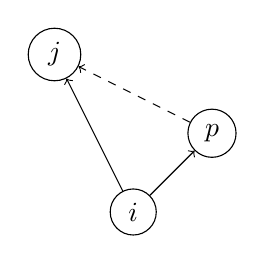
\begin{tikzpicture}
\node[draw,circle] at (0,0) (j) {$j$};
\node[draw,circle] at (1,-2) (i) {$i$};
\node[draw,circle] at (2,-1) (p) {$p$};
\draw[->] (i)--(j);
\draw[->] (i)--(p);
\draw[->,dashed] (p)--(j);
\end{tikzpicture}
}
\end{frame}


\begin{frame}
\frametitle{The Niche Model}
\begin{tikzpicture}
\draw (0,0)--(10,0)
node[anchor = west] {$n$};
\draw (0,.2)--(0,-.2)
node[anchor = north] {$0$};
\draw (10,.2)--(10,-.2)
node[anchor = north] {$1$};
%Predator
\fill (7,0) circle (.07) 
node[anchor = north]  {$n_j$};
%Predator Diet
\draw (7,0)--(7,.75)--(2,.75)--(2,.5);
\draw (.3,0) -- (.3,.5) -- (3.7,.5) -- (3.7,0);
\draw[dashed] (2,.5) -- (2,0) 
node[anchor = south east] {$c_j$};
\draw[<->] (.3,-.5) -- (3.7,-.5)
node[fill=white,pos = 0.5] {$r_j$}; 
\draw[dashed] (.3,0)--(.3,-.55);
\draw[dashed] (3.7,0)--(3.7,-.55);
%Prey
\fill (3,0) circle (.07) 
node[anchor = north west]  {$n_i$};
\draw(4.2,-2) circle (.3)
node {$i$};
\draw[->] (4.5,-2) -- (5.5,-2);
\draw(5.8,-2) circle (.3)
node {$j$};
\end{tikzpicture}
\end{frame}

\subsection{Models}

\begin{frame}
\frametitle{The Allometric Trophic Network (ATN) Model}
***Non Dimensional
\begin{equation}\label{eq:ATNAAAI}
\begin{array}{r l}
\frac{dB_{i}}{dt} &= r_{i}\left(1-\frac{\sum_{j\in \text{basal}}B_{j}}{K}\right)B_{i}\\[1ex]
& - x_{i}B_{i}\\[1ex]
& + x_{i}B_{i}\sum_{j \in \text{diet}(i)}F_{ji}y\\[1ex]
& - \sum_{j \in \text{pred}(i)}x_{j}B_{j}F_{ij}y/e_{ij} \\[1ex]
\end{array}
\end{equation}

and

\begin{equation}\label{eq:FRAAAI}
F_{ij} = \frac{\omega_{ij}B_{i}^{h}}{B_{0}^{h}+ \sum_{k\in \text{diet}(j)}\omega_{kj}B_{k}^{h}}
\end{equation}
\end{frame}

\begin{frame}
\frametitle{Allometry in the ATN}
\begin{itemize}[<+->]
\item A 'middle' road
\item Punchline:
\[
x_i=a_xM_i^{-0.25}
\]
\item i.e. measuring mass vs. attack rates
\end{itemize}
\end{frame}

\subsection{From Structure to Parameters}


\begin{frame}
\frametitle{Allometric Scaling}
\begin{itemize}[<+->]
\item From many parameters, one
\item $x_i = a_xM_i^{-0.25}$
\end{itemize}
\end{frame}

\begin{frame}
\frametitle{Consumer - Resource Body Size Ratio}
\begin{itemize}[<+->]
\item Use trophic levels:
\[
M_i=Z^{TL_i-1}
\]
\item Defines an 'average' size hierarchy.
\end{itemize}
\end{frame}

\begin{frame}
\frametitle{Body Size Hierarchy}
$Z = 10$ (no parasites):
\only<1>{
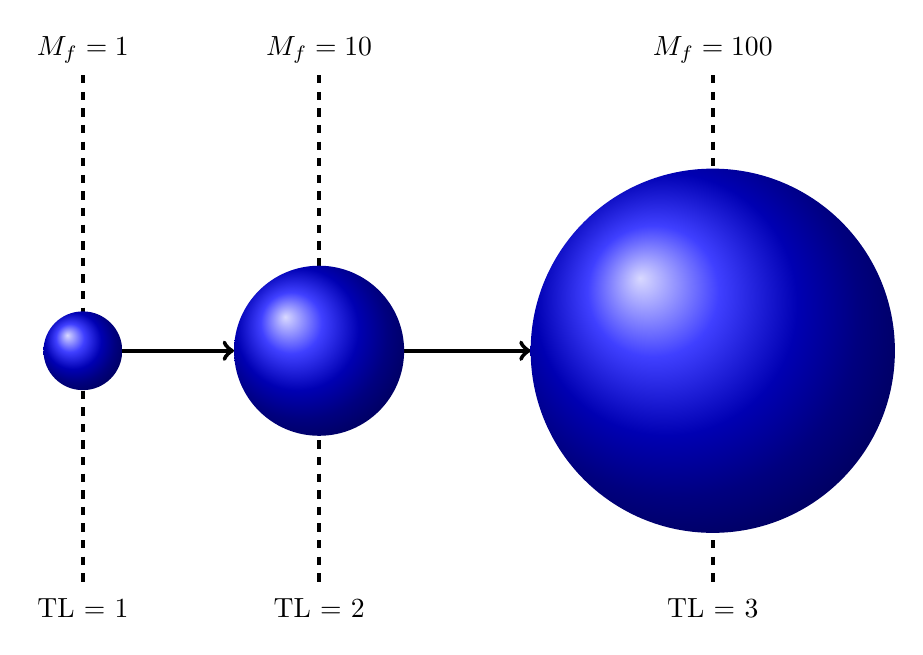
\begin{tikzpicture}
\draw[->,ultra thick] (.5,-1) -> (1.92,-1);
\draw[->,ultra thick] (4.08,-1) -> (5.687,-1);
\draw [ultra thick, dashed] (8,2.5) node [anchor = south]  {$M_f = 100$}--(8,-4) node [anchor = north] {TL = 3};
\draw [ultra thick, dashed] (3,2.5) node [anchor = south]  {$M_f = 10$}--(3,-4) node [anchor = north] {TL = 2};
\draw [ultra thick, dashed] (0,2.5) node [anchor = south]  {$M_f = 1$}--(0,-4) node [anchor = north] {TL = 1};
\shade [ball color=blue] (0,-1) circle (.5cm);
\shade [ball color=blue] (3,-1) circle (1.08cm);
\shade [ball color=blue] (8,-1) circle (2.313cm);
\end{tikzpicture}
}
\only<2>{
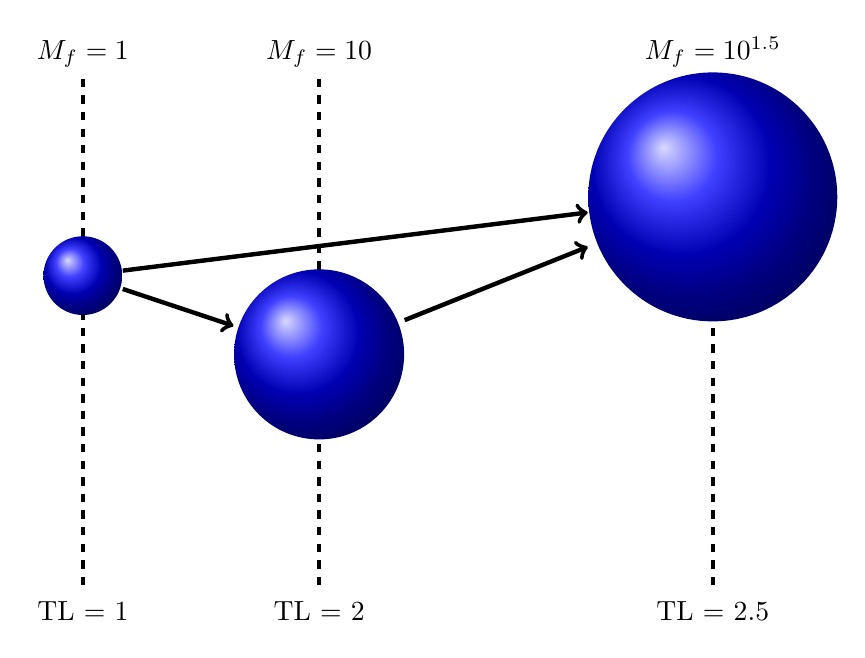
\begin{tikzpicture}
\node [inner sep = .5cm] (s1) at (0,0) {};
\node [inner sep = 1.08cm] (s2) at (3,-1) {};
%\node [inner sep = 2.313cm] (s3) at (8,1) {};
\node [inner sep = 1.581cm] (s4) at (8,1) {};
\draw[->,ultra thick] (s1) -> (s2);
%\draw[->,ultra thick] (s2) -> (s3);
\draw[->,ultra thick](s1) -> (s4);
\draw[->,ultra thick](s2) -> (s4);
\draw [ultra thick, dashed] (8,2.5) node [anchor = south]  {$M_f = 10^{1.5}$}--(8,-4) node [anchor = north] {TL = 2.5};
%\draw [ultra thick, dashed] (8,2.5) node [anchor = south]  {$M_f = 100$}--(8,-4) node [anchor = north] {TL = 3};
\draw [ultra thick, dashed] (3,2.5) node [anchor = south]  {$M_f = 10$}--(3,-4) node [anchor = north] {TL = 2};
\draw [ultra thick, dashed] (0,2.5) node [anchor = south]  {$M_f = 1$}--(0,-4) node [anchor = north] {TL = 1};
\shade [ball color=blue] (s1) circle (.5cm);
\shade [ball color=blue] (s2) circle (1.08cm);
%\shade [ball color=blue] (s3) circle (2.313cm);
\shade [ball color=blue] (s4) circle (1.581cm);
\end{tikzpicture}
}
\end{frame}

\begin{frame}
\frametitle{Consumer - Resource Body Size Ratio}
\begin{itemize}[<+->]
\item Want parasites $Z_p$ times host and free livers $Z_p$ times resource.
\item $i$ free liver:
\[
M_i=Z_f^{TL_i-1}
\]
\item $i$ parasite:
\only<2>{
Maybe...?

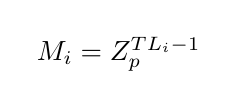
\begin{tikzpicture}
\node at (0,0) {$M_i = Z_p^{TL_i-1}$};
\end{tikzpicture}}

\only<3>{
Wrong!

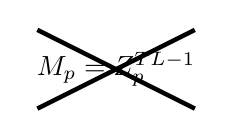
\begin{tikzpicture}
\node at (0,0) {$M_p = Z_p^{TL-1}$};
\draw [ultra thick] (-1,.5) -- (1,-.5);
\draw [ultra thick] (-1,-.5) -- (1,.5);
\end{tikzpicture}}
\end{itemize}
\end{frame}
\begin{frame}
\frametitle{Body Size Hierarchy}
$Z_f = 10$ and $Z_p = 10^{-3}$
\only<1>{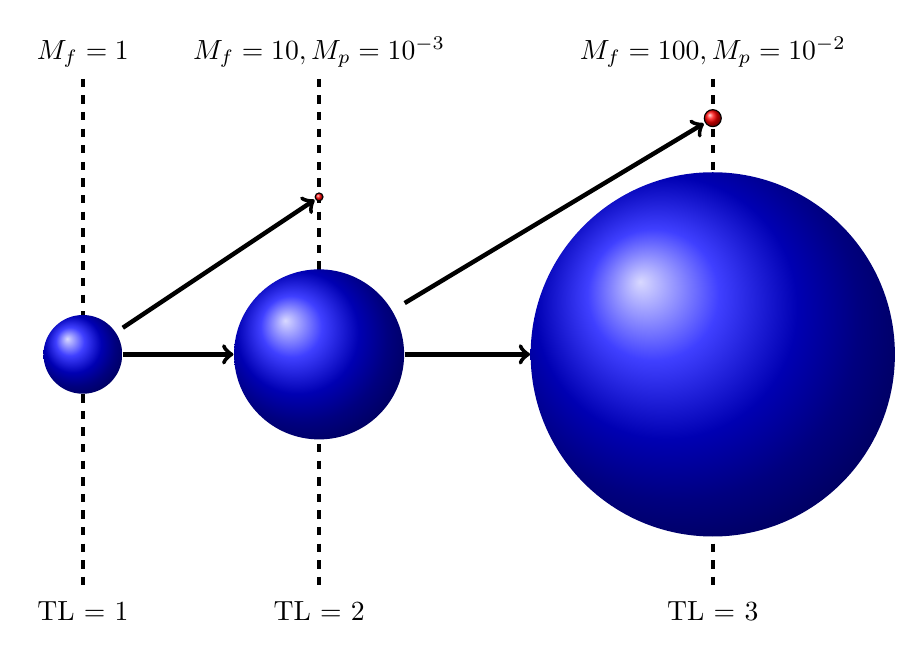
\begin{tikzpicture}
\node [inner sep = .05cm] (p1) at (3,1) {};
\node [inner sep = .108cm] (p2) at (8,2) {};
\node [inner sep = .5cm] (s1) at (0,-1) {};
\node [inner sep = 1.08cm] (s2) at (3,-1) {};
\node [inner sep = 2.313cm] (s3) at (8,-1) {};
\draw[->,ultra thick] (s1) -> (s2);
\draw[->,ultra thick] (s2) -> (s3);
\draw [ultra thick, dashed] (8,2.5) node [anchor = south]  {$M_f = 100,M_p=10^{-2}$}--(8,-4) node [anchor = north] {TL = 3};
\draw [ultra thick, dashed] (3,2.5) node [anchor = south]  {$M_f = 10,M_p=10^{-3}$}--(3,-4) node [anchor = north] {TL = 2};
\draw [ultra thick, dashed] (0,2.5) node [anchor = south]  {$M_f = 1$}--(0,-4) node [anchor = north] {TL = 1};
\draw[->,ultra thick] (s1) -> (p1);
\draw[->,ultra thick] (s2) -> (p2);
%\draw[->,dashed,thick,red] (p1) -> (p2);
%\draw[->,dashed,thick,green] (p1) -> (s3);
\shade [ball color=blue] (s1) circle (.5cm);
\shade [ball color=blue] (s2) circle (1.08cm);
\shade [ball color=blue] (s3) circle (2.313cm);
\draw [ball color=red] (p1) circle (.05cm);

\draw [ball color = red] (p2) circle (.108cm);
\end{tikzpicture}
}
\only<2>{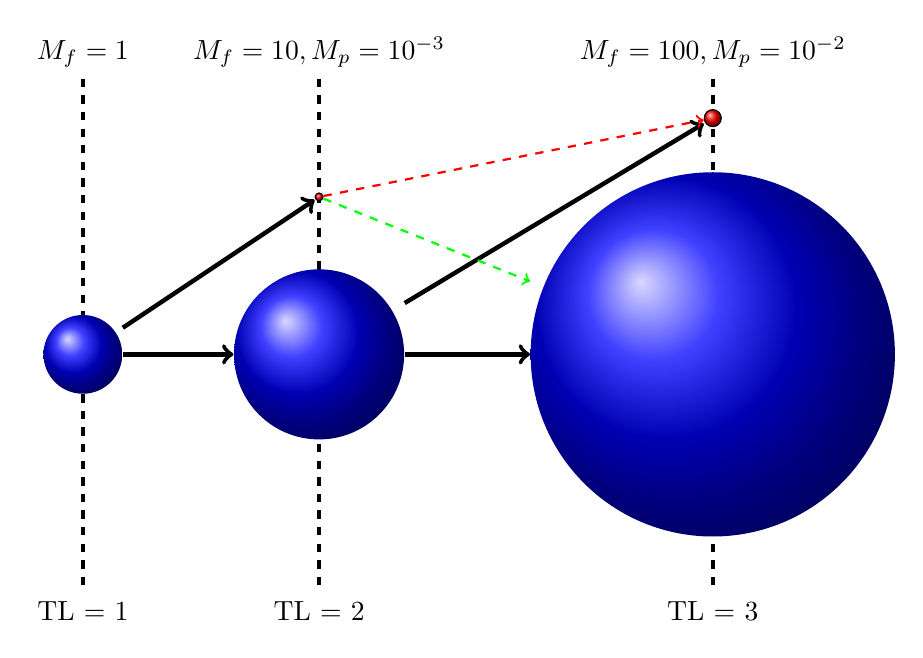
\begin{tikzpicture}
\node [inner sep = .05cm] (p1) at (3,1) {};
\node [inner sep = .108cm] (p2) at (8,2) {};
\node [inner sep = .5cm] (s1) at (0,-1) {};
\node [inner sep = 1.08cm] (s2) at (3,-1) {};
\node [inner sep = 2.313cm] (s3) at (8,-1) {};
\draw[->,ultra thick] (s1) -> (s2);
\draw[->,ultra thick] (s2) -> (s3);
\draw [ultra thick, dashed] (8,2.5) node [anchor = south]  {$M_f = 100,M_p=10^{-2}$}--(8,-4) node [anchor = north] {TL = 3};
\draw [ultra thick, dashed] (3,2.5) node [anchor = south]  {$M_f = 10,M_p=10^{-3}$}--(3,-4) node [anchor = north] {TL = 2};
\draw [ultra thick, dashed] (0,2.5) node [anchor = south]  {$M_f = 1$}--(0,-4) node [anchor = north] {TL = 1};
\draw[->,ultra thick] (s1) -> (p1);
\draw[->,ultra thick] (s2) -> (p2);
\draw[->,dashed,thick,red] (p1) -> (p2);
\draw[->,dashed,thick,green] (p1) -> (s3);
\shade [ball color=blue] (s1) circle (.5cm);
\shade [ball color=blue] (s2) circle (1.08cm);
\shade [ball color=blue] (s3) circle (2.313cm);
\draw [ball color=red] (p1) circle (.05cm);
\draw [ball color = red] (p2) circle (.108cm);
\end{tikzpicture}

}
\end{frame}

\begin{frame}
\frametitle{Consumer - Resource Body Size Ratio}
\begin{itemize}[<+->]
\item If $p$ and $k$: exponents of body size ratios of parasite-host and consumer-resource relationships..
\item $i$ free liver:
\[
M_i = 10^{k(TL_i-1)}
\]
\item $i$ parasite:
\[
M_i = 10^{p + k(TL_i-2)}
\]
\end{itemize}
\end{frame}

\section{Changing the Structure}
\begin{frame}
\frametitle{Inverse Niche Models}
\only<1>{
\begin{tikzpicture}
\draw (0,0)--(10,0)
node[anchor = west] {$n$};
\draw (0,.2)--(0,-.2)
node[anchor = north] {$0$};
\draw (10,.2)--(10,-.2)
node[anchor = north] {$1$};
%Predator
\fill (7,0) circle (.07) 
node[anchor = north]  {$n_j$};
%Predator Diet
\draw (7,0)--(7,.75)--(2,.75)--(2,.5);
\draw (.3,0) -- (.3,.5) -- (3.7,.5) -- (3.7,0);
\draw[dashed] (2,.5) -- (2,0) 
node[anchor = south east] {$c_j$};
\draw[<->] (.3,-.5) -- (3.7,-.5)
node[fill=white,pos = 0.5] {$r_j$}; 
\draw[dashed] (.3,0)--(.3,-.55);
\draw[dashed] (3.7,0)--(3.7,-.55);
%Prey
\fill (3,0) circle (.07) 
node[anchor = north west]  {$n_i$};
\draw(4.2,-2) circle (.3)
node {$i$};
\draw[->] (4.5,-2) -- (5.5,-2);
\draw(5.8,-2) circle (.3)
node {$j$};
\end{tikzpicture}
}
\only<2->{
\begin{tikzpicture}
\draw (0,0)--(10,0)
node[anchor = west] {$n$};
\draw (0,.2)--(0,-.2)
node[anchor = north] {$0$};
\draw (10,.2)--(10,-.2)
node[anchor = north] {$1$};
%Host
\fill (6,0) circle (.07) 
node[anchor = north]  {$n_i$};
%Predator Diet
\draw (7,0.5)--(7,.75)--(2,.75)--(2,0);
\draw (5.3,0) -- (5.3,.5) -- (8.7,.5) -- (8.7,0);
\draw[dashed] (7,.5) -- (7,0) 
node[anchor = south east] {$c_p$};
\draw[<->] (5.3,-.5) -- (8.7,-.5)
node[fill=white,pos = 0.5] {$r_p$}; 
\draw[dashed] (5.3,0)--(5.3,-.55);
\draw[dashed] (8.7,0)--(8.7,-.55);
%Parasite
\fill (2,0) circle (.07) 
node[anchor = north west]  {$n_p$};
\draw(4.2,-2) circle (.3)
node {$i$};
\draw[->] (4.5,-2) -- (5.5,-2);
\draw(5.8,-2) circle (.3)
node {$p$};
\end{tikzpicture}
}
\begin{itemize}
\item<3-> $n_p \sim U(\textcolor{red}{a,b})$
\item<4-> $y_p \sim \text{Beta}(1,\textcolor{red}{\beta_p})$
\item<5-> $r_p \sim \textcolor{red}{(1-n_p)} \cdot y_p$
\item<6-> $c_{p}\sim U(\max{(n_p,r_p/2)},1-r_p/2)$
\end{itemize}
\end{frame}

\begin{frame}
\frametitle{Inverse Niche Models: Further Issues}
\begin{itemize}
\item <1-> Types of links; sub-web connectances
\item <2-> Diet intersections with parasitic niches
\item <3-> Scale dependent errors vs. Parasitic errors
\item <4-> Low(?) parasitic resolution
\end{itemize}
\end{frame}

\subsection{Proposed Models}
\begin{frame}
\frametitle{Host Refuge Model}
Tracking where parasites are, in the simplest way:
\begin{equation}
\phi_i = 
\left\{
\begin{array}{c c c}
\phi & \text{if} & i:\text{ parasite}\\
1 & \text{if} & i:\text{ free-liver}\\
\end{array}
\right.
\end{equation}
\end{frame}

\begin{frame}
\frametitle{Host Refuge Model}
ATN Equations
\begin{align*}
\frac{dB_{b}}{dt} &= r_bB_b\left(1-\frac{\sum_{k\in\text{basal}}B_k}{K}\right) - \sum_k\phi_kB_kx_k\frac{y_{bk}F_{bk}^\text{(troph)}}{e_{bk}} - \sum_k(1-\phi_k)B_kx_k\frac{y_{bk}F^\text{(para)}_{bk}}{e_{bk}}\\
\frac{dB_{c}}{dt} &= -x_cB_c + \phi_cx_cB_c\sum_ky_{kc}F^\text{(troph)}_{kc} + (1-\phi_c)x_cB_c\sum_ky_{kc}F^\text{(para)}_{kc} \\
&- \sum_k \phi_kx_kB_k\frac{y_{ck}F^\text{(troph)}_{ck}}{e_{ck}} - \sum_k (1-\phi_k)x_kB_k\frac{y_{ck}F^\text{(para)}_{ck}}{e_{ck}}\\
\end{align*}
\end{frame}

\begin{frame}
\frametitle{Host Refuge Model}
Functional Responses:

\begin{equation}
F_{ij}^\text{(troph)} = \frac{\omega_{ij}^{(troph)}(\phi_iB_i)^{1+h}}{B_0^{1+h} + \sum_k\omega^\text{(troph)}_{kj}(\phi_kB_k)^{1+h}} 
\end{equation}
and
\begin{equation}
F_{ij}^\text{(para)} = \frac{\omega_{ij}^{(para)}(\phi_iB_i)^{1+h}}{B_0^{1+h} + \sum_k\omega^\text{(para)}_{kj}(\phi_kB_k)^{1+h}} 
\end{equation}
\end{frame}

\begin{frame}
\frametitle{Concomittant Predation}

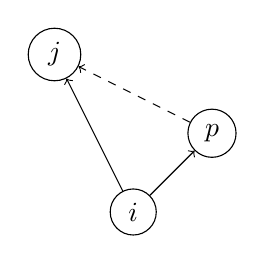
\begin{tikzpicture}
\node[draw,circle] at (0,0) (j) {$j$};
\node[draw,circle] at (1,-2) (i) {$i$};
\node[draw,circle] at (2,-1) (p) {$p$};
\draw[->] (i)--(j);
\draw[->] (i)--(p);
\draw[->,dashed] (p)--(j);
\end{tikzpicture}

Additional loss term to parasitic equations.

\end{frame}

\begin{frame}
\frametitle{Concomittant Predation}
For a parasite, $p$ and host, $h$:
\begin{align*}
I_p & = \sum_h a_{ph}C_h\\
a_{ph}& = \frac{B_p}{B_h}\frac{y_{hp}F_{hp}}{\sum_{k}y_{kp}F_{kp}}\\ 
C_h &= \sum_kx_kB_k\frac{F_{kh}y_{kh}}{e_{kh}} 
\end{align*}
When I don't track parasites inside or outside of hosts. 
\end{frame}

\begin{frame}
\frametitle{Concomittant Predation}
\begin{align*}
I_p & = \sum_h a_{ph}C_h\\
a_{ph} &= \frac{B_p}{B_h}\frac{y_{hp}F_{hp}}{\sum_{k}y_{kp}F_{kp}} \label{aph2}
C_h &= \sum_kx_kB_k\frac{F^\text{(troph)}_{kh}y_{kh}}{e_{kh}} 
\end{align*}
When I do track parasites inside or outside of hosts.
\end{frame}

\section{Results}

\begin{frame}
\frametitle{Empirical Data}
\includegraphics[width = \linewidth]{corMapSpear.jpg}

\end{frame}


\begin{frame}
\frametitle{Empirical Data }
$P$-values for testing $\mu_{free} - \mu_{para}\neq0$ for each property:\vspace{.25in}

\tiny{
\begin{tabular}{|r| c c c c c c|}
\hline
\input{pValsAllProps2.textab}
\hline
\end{tabular}}
\end{frame}

\begin{frame}
\frametitle{A Classification Tree}
\begin{itemize}[<+->]
\item Binary Splits
\item 4 classes
\item Species Overlap?
\item How to use?
\end{itemize}
\end{frame}

\begin{frame}
\frametitle{A Classification Tree}
\begin{tikzpicture}
\tikzstyle{every node}=[draw,rectangle]
\node [] at (0,0) (A) {\tiny
\begin{tabular}{c|c}
Class&Count\\
\hline
1&310\\
2&79\\
3&160\\
4&260\\
\hline
error&61.7\%\\
\end{tabular}
};
\node at (-1.5,-3) (B) {\tiny\begin{tabular}{c|c}
Class&Count\\
\hline
1&213\\
2&3\\
3&22\\
4&2\\
\hline
error&11.2\%\\
\end{tabular}
};
\node at (6,0) (C) {\tiny\begin{tabular}{c|c}
Class&Count\\
\hline
1&97\\
2&76\\
3&138\\
4&258\\
\hline
error&54.6\%\\
\end{tabular}
};
\node at (1.5,-3) (D) {\tiny\begin{tabular}{c|c}
Class&Count\\
\hline
1&18\\
2&3\\
3&2\\
4&119\\
\hline
error&16.1\%\\
\end{tabular}
};
\node at (6,-3) (E) {\tiny\begin{tabular}{c|c}
Class&Count\\
\hline
1&79\\
2&73\\
3&136\\
4&139\\
\hline
error&67.4\%\\
\end{tabular}
};
\node at (2,-6) (F) {\tiny\begin{tabular}{c|c}
Class&Count\\
\hline
1&59\\
2&64\\
3&119\\
4&27\\
\hline
error&55.8\%\\
\end{tabular}
};
\node at (7.5,-6) (G) {\tiny\begin{tabular}{c|c}
Class&Count\\
\hline
1&20\\
2&9\\
3&17\\
4&112\\
\hline
error&29.1\%\\
\end{tabular}
};
\draw[->] (A)-- node [pos = 0.5,fill =white] {\tiny$swTL <2.91$} (B);
\draw[->] (A)--node [pos = 0.5,fill =white] {\tiny$swTL \geq2.91$}(C);
\draw[->] (C)--node [pos = 0.5,fill =white] {\tiny$\langle genPred \rangle <.124$}(D);
\draw[->] (C)--node [pos = 0.5,fill =white] {\tiny$\langle genPred \rangle \geq.124$}(E);
\draw[->] (E)--node [pos = 0.5,fill =white] {\tiny$\langle genPred \rangle <2.38$}(F);
\draw[->] (E)--node [pos = 0.5,fill =white] {\tiny$\langle genPred \rangle \geq 2.38$}(G);
\only<1>{\node [blue] at (-1,-5) (Key) {\tiny
\begin{tabular}{c |l}
Number&Class\\
\hline
1&Ecto. Inv.\\
2&Ecto. Vert.\\
3&Endotherm\\
4&Parasite
\end{tabular}};}
\only<2>{
\node [blue] at (-1.2,-5) {\tiny
\begin{tabular}{c| l| l}
Split& Error & Var. Exp.\\
\hline
0&.617&-\\
1&.418&.323\\
2&.418&0\\
3&.304&.184\\
\end{tabular}
};}
\end{tikzpicture}
\end{frame}

\begin{frame}
\frametitle{Persistence of All Species}

\begin{tikzpicture}
\begin{axis}[x = 15cm,
			title = {All Species Persistence},
		    xlabel = {Fraction Consumers as parasites},
			ylabel = {Persistence}]
\addplot+[
		  only marks, mark = o,
          error bars/.cd,
		  y explicit, y dir=both,
]
table[x =x,y =y,y error =yp,col sep = comma]{plotData/persistence-small-big-subplot-1};
\addlegendentry{\tiny Null Model}
\addplot+[
		  only marks, mark = triangle,
          error bars/.cd,
		  y explicit, y dir=both,
]
table[x =x,y =y,y error =yp,col sep = comma]{plotData/persistence-small-big-subplot-2};
\addlegendentry{\tiny Host Refuge}
\addplot+[
		  only marks, mark = square,
          error bars/.cd,
		  y explicit, y dir=both,
]
table[x =x,y =y,y error =yp,col sep = comma]{plotData/persistence-small-big-subplot-3};
\addlegendentry{\tiny Concomittant Only}
\addplot+[
		  only marks, mark = diamond,
          error bars/.cd,
		  y explicit, y dir=both,
]
table[x =x,y =y,y error =yp,col sep = comma]{plotData/persistence-small-big-subplot-4};
\addlegendentry{\tiny Refuge with Concomittant}
\end{axis}
\end{tikzpicture}
\end{frame}
\begin{frame}
\frametitle{Persistence of Free-Livers}

\begin{tikzpicture}
\begin{axis}[x = 15cm,
			title = {Free Liver Persistence},
		    xlabel = {Fraction Consumers as parasites},
			ylabel = {Persistence}]
\addplot+[
		  only marks, mark = o,
          error bars/.cd,
		  y explicit, y dir=both,
]
table[x =x,y =y,y error =yp,col sep = comma]{plotData/free-persistence-small-big-subplot-1};
\addlegendentry{\tiny Null Model}
\addplot+[ only marks, mark = triangle,
          error bars/.cd,
		  y explicit, y dir=both,
]
table[x =x,y =y,y error =yp,col sep = comma]{plotData/free-persistence-small-big-subplot-2};
\addlegendentry{\tiny Host Refuge}
\addplot+[
		  only marks, mark = square,
          error bars/.cd,
		  y explicit, y dir=both,
]
table[x =x,y =y,y error =yp,col sep = comma]{plotData/free-persistence-small-big-subplot-3};
\addlegendentry{\tiny Concomittant Only}
\addplot+[
		  only marks, mark = diamond,
          error bars/.cd,
		  y explicit, y dir=both,
]
table[x =x,y =y,y error =yp,col sep = comma]{plotData/free-persistence-small-big-subplot-4};
\addlegendentry{\tiny Refuge with Concomittant}
\end{axis}
\end{tikzpicture}
\end{frame}

\begin{frame}
\frametitle{Persistence of Parasites}

\begin{tikzpicture}
\begin{axis}[x = 15cm,
			title = {Parasite Persistence},
		    xlabel = {Fraction Consumers as parasites},
			ylabel = {Persistence},
		    legend pos = north west]
\addplot+[
		  only marks, mark = o,
          error bars/.cd,
		  y explicit, y dir=both,
]
table[x =x,y =y,y error =yp,col sep = comma]{plotData/para-persistence-small-big-subplot-1};
\addlegendentry{\tiny Null Model}
\addplot+[
		  only marks, mark = triangle,
          error bars/.cd,
		  y explicit, y dir=both,
]
table[x =x,y =y,y error =yp,col sep = comma]{plotData/para-persistence-small-big-subplot-2};
\addlegendentry{\tiny Host Refuge}
\addplot+[
		  only marks, mark = square,
          error bars/.cd,
		  y explicit, y dir=both,
]
table[x =x,y =y,y error =yp,col sep = comma]{plotData/para-persistence-small-big-subplot-3};
\addlegendentry{\tiny Concomittant Only}
\addplot+[
		  only marks, mark = diamond,
          error bars/.cd,
		  y explicit, y dir=both,
]
table[x =x,y =y,y error =yp,col sep = comma]{plotData/para-persistence-small-big-subplot-4};
\addlegendentry{\tiny Refuge with Concomittant}
\end{axis}
\end{tikzpicture}
\end{frame}


\begin{frame}
\frametitle{Fraction of Species Extinct Before Parasites}

\begin{tikzpicture}
\begin{axis}[x = 15cm,
		    xlabel = {Fraction Consumers as parasites},
			ylabel = {$Fraction of Species$},
		    legend pos = north east]
\addplot+[
		  only marks, mark = o,
          error bars/.cd,
		  y explicit, y dir=both,
]
table[x =x,y =y,y error =yp,col sep = comma]{plotData/frac-para-first-small-big-subplot-1};
\addlegendentry{\tiny Null Model}
\addplot+[
		  only marks, mark = triangle,
          error bars/.cd,
		  y explicit, y dir=both,
]
table[x =x,y =y,y error =yp,col sep = comma]{plotData/frac-para-first-small-big-subplot-2};
\addlegendentry{\tiny Host Refuge}
\addplot+[
		  only marks, mark = square,
          error bars/.cd,
		  y explicit, y dir=both,
]
table[x =x,y =y,y error =yp,col sep = comma]{plotData/frac-para-first-small-big-subplot-3};
\addlegendentry{\tiny Concomittant Only}
\addplot+[
		  only marks, mark = diamond,
          error bars/.cd,
		  y explicit, y dir=both,
]
table[x =x,y =y,y error =yp,col sep = comma]{plotData/frac-para-first-small-big-subplot-4};
\addlegendentry{\tiny Refuge with Concomittant}
\end{axis}
\end{tikzpicture}
\end{frame}

\begin{frame}
\frametitle{Fraction of Parasitic Links with Host Extinct First}

\begin{tikzpicture}
\begin{axis}[x = 15cm,
		    xlabel = {Fraction Consumers as parasites},
			ylabel = {Fraction of Species},
		    legend pos = south east]
\addplot+[
		  only marks, mark = o,
          error bars/.cd,
		  y explicit, y dir=both,
]
table[x =x,y =y,y error =yp,col sep = comma]{plotData/frac-Host-first-small-big-subplot-1};
\addlegendentry{\tiny Null Model}
\addplot+[
		  only marks, mark = triangle,
          error bars/.cd,
		  y explicit, y dir=both,
]
table[x =x,y =y,y error =yp,col sep = comma]{plotData/frac-Host-first-small-big-subplot-2};
\addlegendentry{\tiny Host Refuge}
\addplot+[
		  only marks, mark = square,
          error bars/.cd,
		  y explicit, y dir=both,
]
table[x =x,y =y,y error =yp,col sep = comma]{plotData/frac-Host-first-small-big-subplot-3};
\addlegendentry{\tiny Concomittant Only}
\addplot+[
		  only marks, mark = diamond,
          error bars/.cd,
		  y explicit, y dir=both,
]
table[x =x,y =y,y error =yp,col sep = comma]{plotData/frac-Host-first-small-big-subplot-4};
\addlegendentry{\tiny Refuge with Concomittant}
\end{axis}
\end{tikzpicture}
\end{frame}


\begin{frame}
\frametitle{Fraction of Links with Consumer extinct First}

\begin{tikzpicture}
\begin{axis}[x = 15cm,
		    xlabel = {Fraction Consumers as parasites},
			ylabel = {Fraction of Parasites},
		    legend pos = south east]
\addplot+[
		  only marks, mark = o,
          error bars/.cd,
		  y explicit, y dir=both,
]
table[x =x,y =y,y error =yp,col sep = comma]{plotData/frac-con-first-small-big-subplot-1};
\addlegendentry{\tiny Null Model}
\addplot+[
		  only marks, mark = triangle,
          error bars/.cd,
		  y explicit, y dir=both,
]
table[x =x,y =y,y error =yp,col sep = comma]{plotData/frac-con-first-small-big-subplot-2};
\addlegendentry{\tiny Host Refuge}
\addplot+[
		  only marks, mark = square,
          error bars/.cd,
		  y explicit, y dir=both,
]
table[x =x,y =y,y error =yp,col sep = comma]{plotData/frac-con-first-small-big-subplot-3};
\addlegendentry{\tiny Concomittant Only}
\addplot+[
		  only marks, mark = diamond,
          error bars/.cd,
		  y explicit, y dir=both,
]
table[x =x,y =y,y error =yp,col sep = comma]{plotData/frac-con-first-small-big-subplot-4};
\addlegendentry{\tiny Refuge with Concomittant}
\end{axis}
\end{tikzpicture}
\end{frame}

%\begin{frame}
%\frametitle{Fraction of Links with Resource Extinct First}
%
%\begin{tikzpicture}
%\begin{axis}[x = 15cm,
%		    xlabel = {Fraction Consumers as parasites},
%			ylabel = {Fraction of Links},
%		    legend pos = north east]
%\addplot+[
%		  only marks, mark = o,
 %         error bars/.cd,
%		  y explicit, y dir=both,
%]
%table[x =x,y =y,y error =yp,col sep = comma]{plotData/frac-res-first-small-big-subplot-1};
%\addlegendentry{\tiny Null Model}
%\addplot+[
%		  only marks, mark = triangle,
%          error bars/.cd,
%		  y explicit, y dir=both,
%]
%table[x =x,y =y,y error =yp,col sep = comma]{plotData/frac-res-first-small-big-subplot-2};
%\addlegendentry{\tiny Host Refuge}
%\addplot+[
%		  only marks, mark = square,
%          error bars/.cd,
%		  y explicit, y dir=both,
%]
%table[x =x,y =y,y error =yp,col sep = comma]{plotData/frac-res-first-small-big-subplot-3};
%\addlegendentry{\tiny Concomittant Only}
%\addplot+[
%		  only marks, mark = diamond,
%          error bars/.cd,
%		  y explicit, y dir=both,
%]
%
%table[x =x,y =y,y error =yp,col sep = comma]{plotData/frac-res-first-small-big-subplot-4};
%\addlegendentry{\tiny Refuge with Concomittant}
%\end{axis}
%\end{tikzpicture}
%\end{frame}

\section{Conclusions}
\begin{frame}
\frametitle{Conclusions}
\begin{itemize}[<+->]
\item Parasites are hard to distinguish structurally
\item What differences there are could be from bias
\item Adding parasites tends to decrease persistence
\item some patterns to which species go extinct
\end{itemize}
\end{frame}


\section{Future Work}
\begin{frame}
\begin{itemize}[<+->]
\item Switching types of species is bad
\item More analysis of structures
\item Equilibrium points and limit cycles
\item Analysis of Equations and parameters
\end{itemize}
\end{frame}

\end{document}
